\section{Theorie}
\label{sec:Theorie}


\begin{figure}
    \centering 
    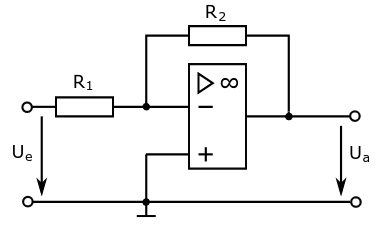
\includegraphics[width=.5\textwidth]{Bilder/Inv_Lin.png}
    \caption{Schaltbild eines invertierenden Integrators.}
    \label{fig:Inv_Lin}
\end{figure}



\begin{figure}
    \centering 
    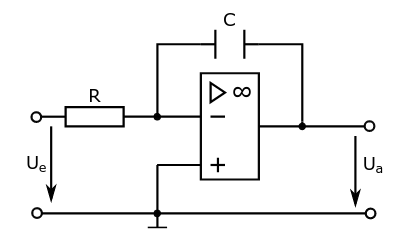
\includegraphics[width=.5\textwidth]{Bilder/Um_Int.png}
    \caption{Schaltbild eines Umker-Integrators.}
    \label{fig:Um_Int}
\end{figure}

\begin{figure}
    \centering 
    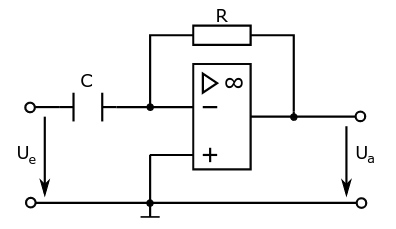
\includegraphics[width=.5\textwidth]{Bilder/Inv_Dif.png}
    \caption{Schaltbild eines invertierenden Differenzierers.}
    \label{fig:Inv_Dif}
\end{figure}

\begin{figure}
    \centering 
    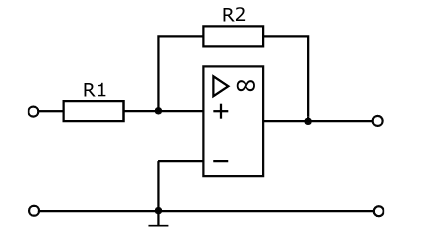
\includegraphics[width=.5\textwidth]{Bilder/Schmitt.png}
    \caption{Schaltbild eines nichtinvertierenden Schmitt-Triggers.}
    \label{fig:Schmitt}
\end{figure}

\begin{figure}
    \centering 
    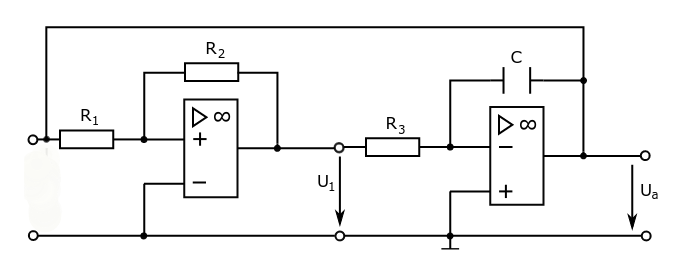
\includegraphics[width=.9\textwidth]{Bilder/Signal.png}
    \caption{Schaltbild eines Signalgenerators aus der Reihe eines nichtinvertierenden Schmitt-Triggers und eines Umker-Integrators.}
    \label{fig:Signal}
\end{figure}
%In knapper Form sind die physikalischen Grundlagen des Versuches, des Messverfahrens, sowie sämtliche für die Auswertung erforderlichen Gleichungen darzustellen. (Keine Herleitung)

%(eventuell die Aufgaben)

%Der Versuchsaufbau: Beschreibung des Versuchs und der Funktionsweise (mit Skizze/Bild/Foto)
